\documentclass[a5paper,headsepline,titlepage,10pt,nnormalheadings,DIVcalc]{scrbook}
\usepackage[a5paper,backref]{hyperref}
%\usepackage{palatino}
\usepackage{graphicx}
\usepackage{wrapfig}
\usepackage[bahasa]{babel}
\usepackage{fancyhdr}

%\setlength{\voffset}{0.5in}
%\setlength{\oddsidemargin}{28pt}
%\setlength{\evensidemargin}{0pt}
\renewcommand{\footrulewidth}{0.5pt}
\lhead[\fancyplain{}{\thepage}]%
      {\fancyplain{}{\rightmark}}
\rhead[\fancyplain{}{\leftmark}]%
      {\fancyplain{}{\thepage}}
\pagestyle{fancy}
\lfoot[\emph{Ziarah Gua Maria Tritis Gunung Kidul}]{}
\rfoot[]{\emph{Lingkungan St Petrus Maguwo}}
\cfoot{}

\newcommand{\BU}[1]{\begin{itemize} \item[U:] #1 \end{itemize}}
\newcommand{\BI}[1]{\begin{itemize} \item[I:] #1 \end{itemize}}
\newcommand{\BP}[1]{\begin{itemize} \item[P:] #1 \end{itemize}}
\title{Jalan Salib Bersama Bunda Maria}
\author{Ziarah Gua Maria Tritis\\Lingkungan St. Petrus Maguwo}
\date{Oktober 2009}
\hyphenation{sa-u-da-ra-ku}
\hyphenation{ke-ri-ngat}
\hyphenation{je-ri-tan}
\hyphenation{hu-bung-an}
\hyphenation{me-nya-dari}
\hyphenation{Eng-kau}
\hyphenation{ke-sa-lah-an}
\hyphenation{ba-gai-ma-na}
\hyphenation{Tu-han}
\hyphenation{di-per-ca-ya-kan}
\hyphenation{men-ja-uh-kan}
\hyphenation{bu-kan-lah}
\hyphenation{per-sa-tu-kan-lah}
\hyphenation{ma-khluk}
\hyphenation{Sem-buh-kan-lah}
\hyphenation{ja-lan}
\hyphenation{mem-bu-tuh-kan}
\hyphenation{be-ri-kan-lah}
\hyphenation{me-ra-sa-kan}
\hyphenation{te-man-ilah}
\hyphenation{mem-bi-ngung-kan}
\hyphenation{di-ka-gum-i}
\hyphenation{ta-ngis-an-Mu}
\hyphenation{mi-lik-ilah}


\begin{document}
\maketitle

\noindent{\textit{Jalan Salib Bersama Bunda Maria ini mengisahkan perjalanan Bumda Maria yang dengan tekun, setia dan perasaan sedih serta pilu yang amat dalam, mengikuti perjalanan Puteranya yang menjalani kematianNya di Kayu Salib. Kita diajak untuk bertekun bersama Bunda Maria dan kita dapat merasakan juga secara langsung bagaimana sedihnya perasaan seorang ibu yang ditinggal mati oleh anaknya dalam kesengsaraan, padahal sang ibu mengetahui bahwa anaknya tidak melakukan satu kesalahaan apapun, namun anaknya rela mati untuk menebus dosa umat manusia, dosa anak-anak keturunan Adam yang harus dibayar dengan "SANGAT MAHAL".}}

\begin{wrapfigure}[0]{r}{2cm}
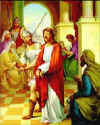
\includegraphics[width=2cm]{jalansalib_files/01_small.jpg}
\end{wrapfigure}
\subsection*{Perhentian I \\
YESUS DI JATUHI HUKUMAN MATI}

\BP{ Kami menyembah Dikau ya Tuhan dan bersyukur\\kepadaMu.}
\BU{ Sebab dengan salib suci, Engkau telah menembus dunia.}

\BP{Hari jumat pagi,aku melihat Puteraku lagi, itulah untuk pertama kali aku melihatDia, sejak para serdadu membawa-Nya pergi. Tubuh-Nya hancur bekas cambukan, pukulan mereka, darah mengalir disekujur tubuhNya. Melihat itu hatiku hancur luluh seakan tersayat pedang sengsara, dan air mataku bercucuran dipipiku.Bagaikan penjahat besar Puteraku dihadapkan kehadapan Pilatus untuk diadili. Pilatus bertanya kepada khalayak banyak mengapa mereka hendak menghukum Puteraku? Semua orang di sekitarku berteriak salibkan Dia!, salibkan Dia!. Aku ingin memohon dengan sangat agar mereka diam.Tetapi aku menyadari,bahwa semuanya itu harus terjadi. Oleh sebab itu aku berdiri tenang dan menangis dalam hatiku diam-diam, sambil berdoa;}

\BU{ Tuhan Yesus Kristus,sulit bagiku untuk membayangkan penderitaan yang IbuMu rasakan. Ketika Engkau dijatuhi hukuman mati. Tetapi apa yang terjadi sekarang atas diriku, apabila saya berbuat dosa...? salibkan Dia". Apa bila saya menaruh dendam, marah, benci?..."salibkan Dia". Apabila saya menghakimi sesama...? "salibkan Dia". Bukankah hal ini menyebabkan Engkau dan ibu-Mu mencurahkan air mata nestapa dan menambah penderitaan-Mu?}
\large\begin{itemize}\item[~]\it{Bapa Kami - Salam Maria}\end{itemize}\normalsize

\BP{Kasihanilah Tuhan, kasihanilah aku}
\BU{Allah ampunilah aku orang berdosa.}

\begin{itemize}\item[~]\textit{
\begin{tabular}{cccccccccc}
&1&2&3&2&3&5&4&3&.\\
1.&Bun-&da&Ye-&sus&yang&ber-&du-&ka\\
&3&2&1&7&6&7&6&5&.\\
&me-&ra-&ta-&pi&Pu-&te-&ra-&nya\\
&2&1&2&3&2&1&1&.    //\\
&di&ka-&ki&sa-&lib&ku-&dus
\end{tabular}}
\end{itemize}


\begin{wrapfigure}[0]{r}{2cm}
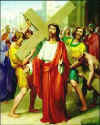
\includegraphics[width=2cm]{jalansalib_files/02_small.jpg}
\end{wrapfigure}
\subsection*{Perhentian II\\
YESUS MEMANGGUL SALIBNYA}


\BP{ Kami menyembah Dikau ya Tuhan dan bersyukur\\kepadaMu.}
\BU{ Sebab dengan salib suci, Engkau telah menembus dunia.}

\BP{ Setelah kekuatanku agak kuat, aku berjalan bersama orang banyak itu, menuju pintu gerbang istana. Pintu terbuka dan Puteraku berjalan keluar terhuyung-huyung, para algojo tertawa ria dibelakang-Nya. Dua lelaki menyeret sebatang kayu salib berat, dan menghempaskanya diatas bahu Yesus. Lalu mereka mendorong Dia dengan kasar dan keji sekali ke jalan yang berbatu-batu. Melihat itu hatiku amat sedih dan taktertahankan lagi. Ingin aku mengambil salib itu dari bahu Puteraku dan menaruhnya diatas bahuku sendiri. Tetapi aku menyadari, bahwa itu semua harus terjadi, maka aku berjalan diam-diam sambil berdoa;}

\BU{ Tuhan Yesus Kristus, ampunilah aku, atas perbuatan dosa yang selama ini aku lakukan, akulah yang menyebabkan engkau memanggul salib itu dan menambah berat salib-Mu, oleh menutup mata terhadap sesamaku yang menderita dan butuh pertolonganku, ampunilah aku karena sering meremehkan orang lain serta menghindar dari orang-orang tertentu yang ingin berbicara denganku.Bantulah aku untuk menjadi seperti ibuMu yang selalu menolong dan meringankan beban salib manusia.}

\large\begin{itemize}\item[~]\it{Bapa Kami - Salam Maria}\end{itemize}\normalsize
\BP{Kasihanilah Tuhan, kasihanilah aku}
   \BU{Allah ampunilah aku orang berdosa.}

\begin{itemize}
\item[2.] \it{Hatinya berkeluh kesah\\ hancur luluh rasa batin\\
    tersayat duka-lara.}
\end{itemize}

\begin{wrapfigure}[0]{r}{2cm}
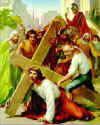
\includegraphics[width=2cm]{jalansalib_files/03_small.jpg}
\end{wrapfigure}
\subsection*{Perhentian III\\
YESUS JATUH PERTAMA KALINYA DIBAWAH\\SALIBNYA}

\BP{ Kami menyembah Dikau ya Tuhan dan bersyukur\\kepadaMu.}
\BU{ Sebab dengan salib suci, Engkau telah menembus dunia.}

\BP{ Aku berada dibelakang dekat Puteraku, ketika Dia berjalan dengan beban salib yang berat menuju kalvari, hatiku pilu dan sangat sedih melihat Dia dalam sengsara sehebat itu.Ia sudah lemah karena penderitaan dan siksaan yang baru dideritaNya.Ia tidak mampu menahan diriNya, tiba-tiba Ia tersungkur dibawah salib. Ketika aku melihat Dia jatuh hatiku hancur luluh, apabila salib berat menimpanya lagi, aku takut, kalau-kalau Puteraku sudah meninggal, lalu algojo-algojo menendang, menarik dan mengolok, tak ada satupun yang menolong, perlahan-lahan Dia bangkit dan meneruskan perjalanan,aku menyadari bahwa semuanya itu harus terjadi,maka aku berjalan dengan pasrah,  menangis dan berdoa diam-diam;}

\BU{ Ya Tuhan, betapa sering aku jatuh di dalam dosa yang sama dan jarang aku sadari, betapa sering aku melihat sesamaku berbuat kesalahan dan aku mentertawakan mereka, kadang aku marah bila sesamaku menyakiti hatiku. Maria turut merasakan jalan salib yang Engkau tempuh. Bantulah aku untuk mengakui dosa dan salahku kepada-Mu, serta turut merasakan penderitaan sesamaku, Tuhan kasihanilah aku.}

\large\begin{itemize}\item[~]\it{Bapa Kami - Salam Maria}\end{itemize}\normalsize
\BP{Kasihanilah Tuhan, kasihanilah aku}
\BU{Allah ampunilah aku orang berdosa.}

\begin{itemize}
\item[3.] \it{Betapa hebat derita\\ menimpa bunda suci\\
   menyaksikan Puteranya}
\end{itemize}

\begin{wrapfigure}[0]{r}{2cm}
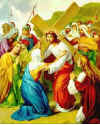
\includegraphics[width=2cm]{jalansalib_files/04_small.jpg}
\end{wrapfigure}
\subsection*{Perhentian IV\\
YESUS BERJUMPA DENGAN BUNDANYA}

\BP{ Kami menyembah Dikau ya Tuhan dan bersyukur\\kepadaMu.}
\BU{ Sebab dengan salib suci, Engkau telah menembus dunia.}

\BP{ Aku lolos menerobos kumpulan orang banyak yang berjalan di samping Puteraku. Dan aku berdiri dipinggir jalan salib yang hendak dilewati oleh Puteraku. Aku memanggil Dia. Ia berhenti. Kami bertukar pandangan, hatiku tidak bisa menahan sedih dan duka yang begitu hebatnya sehingga tak sanggup mengeluarkan satu katapun. Pandangan mataNya mengisyaratkan batinku "Kuatkan hatimu ibu,semua ini ada tujuannya". Lalu Dia berjalan terus terhuyung-huyung. Aku hanya meratap dipelukan para ibu yang berdiri disampingku. Aku berjalan bersama orang banyak dan berdoa diam-diam;}

\BU{Ya Tuhan, ampunilah aku, karena sering sekali aku berpaling dari pada-Mu, kadangkala aku menjauhi-Mu bila aku telah berbuat dosa dan sering kuulang-ulangi perbuatan itu. Ampunilah aku karena banyak sekali aku mengingat-ingat hal-hal yang tak berkenan kepada-Mu dan mudah jatuh lagi dalam dosa yang sama.Aku tak menghiraukan panggilan-Mu untuk tetap teguh dan setia kepada-Mu. Berilah aku hati yang terbuka seperti ibu Maria.}

\large\begin{itemize}\item[~]\it{Bapa Kami - Salam Maria}\end{itemize}\normalsize
\BP{Kasihanilah Tuhan, kasihanilah aku}
   \BU{Allah ampunilah aku orang berdosa.}

\begin{itemize}
\item[4.] \it{Alangkah sedih hatinya\\ memandang siksa
    yang hebat\\ diderita Anaknya
}\end{itemize}

\begin{wrapfigure}[0]{r}{2cm}
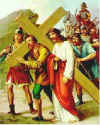
\includegraphics[width=2cm]{jalansalib_files/05_small.jpg}
\end{wrapfigure}
\subsection*{Perhentian V\\
SIMON KIRENE MEMBANTU YESUS\\MEMANGGUL SALIBNYA}

\BP{   Kami menyembah Dikau ya Tuhan dan bersyukur\\kepadaMu.}
\BU{   Sebab dengan salib suci, Engkau telah menembus dunia.}

\BP{ Aku  dapat   melihat  sekarang  rasa  letih  dan  tak  berdaya  terpancar dari wajah Puteraku, salib yang  dipikul-Nya sangat berat, jalannya mendaki. aku melihat setiap langkah Puteraku sepertinya merupakan langkah terakhir. Aku turut menderita bersama-Nya, dan aku melihat suatu perbuatan kejam didekat Puteraku. Algojo-algojo menarik dan memaksa seorang petani untuk membantu memikul salib Puteraku, aku menyaksikan wajah Simon dengan terpaksa dan memalukan untuk memikul palang yang berat itu. Simon bertanya kepada algojo itu, mengapa aku harus membantu Yesus, Puteraku? Aku mengerti maksudnya dan berjalan terus sambil berdoa dalam hatiku;}

\BU{ Tuhan Yesus  Kristus,  kasihanilah aku, karena sudah banyak sekali aku menolak menolong Engkau, melalui sesamaku. Aku hanya mementingkan diriku saja dan sering sangsi akan sabda-Mu yang mengatakan "Sesungguhnya segala sesuatu yang kamu lakukan untuk salah seorang dari saudaraku yang paling hina ini, kamu telah melakukannya untuk Aku". Tuhan, jangan biarkan aku seperti Simon karena terpaksa, tetapi bantulah aku sepertiibu-Mu, Maria, yang selalu mengikuti-Mu dengan setia sampai di bawah salib.}

\large\begin{itemize}\item[~]\it{Bapa Kami - Salam Maria}\end{itemize}\normalsize
\BP{Kasihanilah Tuhan, kasihanilah aku}
   \BU{Allah ampunilah aku orang berdosa.}

\begin{itemize}
\item[5.] \it{Siapa yang tak terharu\\ bila ingat bunda Yesus\\
    tertimpa duka lara.
}\end{itemize}

\begin{wrapfigure}[0]{r}{2cm}
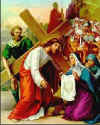
\includegraphics[width=2cm]{jalansalib_files/06_small.jpg}
\end{wrapfigure}
\subsection*{Perhentian VI\\
VERONIKA MENGUSAP WAJAH YESUS}

\BP{   Kami menyembah Dikau ya Tuhan dan bersyukur\\kepadaMu.}
\BU{   Sebab dengan salib suci, Engkau telah menembus dunia.}

\BP{Aku dengan setia mengikuti Puteraku dari dekat sekali, darah dan keringat mengalir di wajahnya ingin sekali aku mau membersihkannya. Tampa aku duga, tiba-tiba seorang wanita yang bersama kami, mendesak maju melewati algojo-algojo. Ia segera mengeluarkan kain putih, mendekati Puteraku dan mengusapi wajah-Nya yang berlumuran darah dan keringat itu. Dengan segera seorang algojo menarik wanita itu kesamping, namun raut wajahnya seakan-akan bertanya" mengapa kamu berbuat demikian terhadap orang ini"?Aku merenungkan dalam hatiku perbuatan cintanya dan aku berjalan terus dalam iman dan sambil berdoa diam-diam.}

\BU{Tuhan  Yesus,  Wanita  itu telah memberikan cintanya yang terbaik kepada-Mu, namun   aku masih ingat diriku sendiri, dan aku telah banyak menerima dari pada-Mu dan sesamaku dari pada yang aku beri. Banyak kesempatan sebenarnya setiap hari bagiku untuk memberi kepada-Mu. Namun aku melalaikannya. Penebusku, bantulah aku untuk memberikan seluruh hidupku kepada-Mu dan mengembalikan milikku kepada-Mu.}

\large\begin{itemize}\item[~]\it{Bapa Kami - Salam Maria}\end{itemize}\normalsize
\BP{Kasihanilah Tuhan, kasihanilah aku}
   \BU{Allah ampunilah aku orang berdosa.}

\begin{itemize}
\item[6.] \it{Hai Bundaku yang pemurah\\beri aku rasa duka\\
    berbagi deritamu.
}\end{itemize}

\begin{wrapfigure}[0]{r}{2cm}
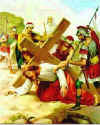
\includegraphics[width=2cm]{jalansalib_files/07_small.jpg}
\end{wrapfigure}
\subsection*{Perhentian VII\\
YESUS JATUH UNTUK KEDUA KALINYA}

\BP{   Kami menyembah Dikau ya Tuhan dan bersyukur\\kepadaMu.}
\BU{   Sebab dengan salib suci, Engkau telah menembus dunia.}

\BP{Yesus merasakan tanaga-Nya sudah habis, dengan tidak disangka-sangka Ia jatuh lagi dibawah salib, kesedihan dan dukacitaku tak dapat kutahan lagi, kepalaNya tertelungkup ke tanah, aku berpikir, mungkin Dia sudah meninggal. Namun dengan tenaga yang masih tersisa, Puteraku berusaha berdiri kembali untuk menyelesaikan kurban-Nya, hatiku hancur luluh melihat ketidak berdayaan Puteraku yang berjalan kembali. Namun aku menyadari harus terjadi, maka aku berjalan dibelakang Puteraku dengan diam-diam kupanjatkan doa sambil menangis.}

\BU{Ya Tuhan, aku sering  jatuh  dengan  kesalahan dan dosa yang sama, kadang aku enggan untuk kembali kepada-Mu mengakui kesalahan atas dosa-dosaku sehingga menyebabkan Engkau jatuh lagi. Berilah aku semangat untuk memulai merubah diri dan mengambil langkah yang baik untuk menghidari dosa dan kesalahan-kesalahan yang merugikan Dikau dan sesamaku. Aku mohon kepada-Mu, ampunilah aku.}

\large\begin{itemize}\item[~]\it{Bapa Kami - Salam Maria}\end{itemize}\normalsize
\BP{Kasihanilah Tuhan, kasihanilah aku}
   \BU{Allah ampunilah aku orang berdosa.}

\begin{itemize}
\item[7.] \it{Nyalakan dalam hatiku\\ kasih Kristus yang
    sejati\\pantas jadi saksiNya.
}\end{itemize}

\begin{wrapfigure}[0]{r}{2cm}
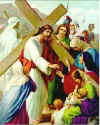
\includegraphics[width=2cm]{jalansalib_files/08_small.jpg}
\end{wrapfigure}
\subsection*{Perhentian VIII\\
YESUS MENGHIBUR WANITA-WANITA YANG\\MENANGIS}
\BP{   Kami menyembah Dikau ya Tuhan dan bersyukur\\kepadaMu.}
\BU{   Sebab dengan salib suci, Engkau telah menembus dunia.}

\BP{Aku  berjalan  di belakang Puteraku,  ketika  aku melihat  Dia berhenti, di tengah kumpulan wanita   yang meratapi Dia, dan menaruh belas kasihan kepada-Nya. Mereka diberi kesempatan menerima Dia sebagai Mesias, namun seperti banyak orang lain, mereka menolak PuteraKu, PuteraKu mengatakan kepada mereka, agar mereka menangisi diri mereka dan dosa-dosa yang membawa pertobatan, namun mereka tidak melihat hubungan kata-kata Puteraku itu dengan jalan salib dan wafat-Nya.Tapi aku mengerti dan ketika Dia meneruskan jalan salib-Nya,aku berdoa dalam hati dan terus mengikuti-Nya dengan diam-diam.}

\BU{Penyelamatku, banyak  sekali  aku  telah berlaku seperti wanita-wanita ini, selalu melihat kesalahan pada orang lain, dan menaruh kasihan pada orang yang bersalah itu, tapi amat jarang aku melihat kesalahan pada diriku atas dosa dan tingkah lakuku. Tuhan aku mohon belas kasihan-Mu, ampunilah aku karena perbuatanku selama ini tidak berkenan kepada-Mu, ajarilah aku untuk sungguh-sungguh bertobat.}

\large\begin{itemize}\item[~]\it{Bapa Kami - Salam Maria}\end{itemize}\normalsize
\BP{Kasihanilah Tuhan, kasihanilah aku}
   \BU{Allah ampunilah aku orang berdosa.}

\begin{itemize}
\item[8.] \it{Lukiskan ya Bunda suci\\luka Yesus yang berdarah\\
    dalam lubuk hatiku
}\end{itemize}

\begin{wrapfigure}[0]{r}{2cm}
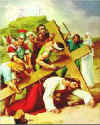
\includegraphics[width=2cm]{jalansalib_files/09_small.jpg}
\end{wrapfigure}
\subsection*{Perhentian IX\\
YESUS JATUH KETIGA KALINYA DIBAWAH SALIB}

\BP{    Kami menyembah Dikau ya Tuhan dan bersyukur\\kepadaMu.}
\BU{   Sebab dengan salib suci, Engkau telah menembus dunia.}

\BP{Puncak  gunung  Golgolta  sudah  tampak,Puteraku sudah tidak punya tenaga lagi dan para Algojo berpekik sorak memperlakukan Yesus Puteraku dengan kejam, kasar dan mendorong Dia. Puteraku terjatuh ketiga kalinya, Dia jatuh di atas batu-batu dan salib berat menimpaNya. Sengsaraku semakin dahsyat melihatNya mereka hampir-hampir menyeret Dia pada bagian akhir perjalanNya itu, hatiku hancur luluh membayangkan apa yang akan mereka perbuat lagi terhadap Puteraku itu. Namun aku menyadari semua ini harus terjadi. Hanya doa dan tangisan yang dapat kulakukan dengan diam-diam.}

\BU{Yesusku yang terkasih, cinta-Mu begitu besar atas diriku, Engkau sengsara demi aku orang  yang berdosa ini. Ampunilah aku Tuhan, atas dosa yang aku perbuat selama ini yang menyebabkan Engkau jatuh. Bantulah aku ya Tuhan agar aku selalu dekat pada-Mu seperti ibu Maria yang tak henti mengikuti-Mu.}

\large\begin{itemize}\item[~]\it{Bapa Kami - Salam Maria}\end{itemize}\normalsize
\BP{Kasihanilah Tuhan, kasihanilah aku}
   \BU{Allah ampunilah aku orang berdosa.}

\begin{itemize}
\item[9.] \it{Beri aku sebagian\\ dari siksa suci Yesus\\
    agar dapat kutiru.
}\end{itemize}

\begin{wrapfigure}[0]{r}{2cm}
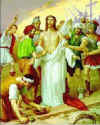
\includegraphics[width=2cm]{jalansalib_files/10_small.jpg}
\end{wrapfigure}
\subsection*{Perhentian X\\
PAKAIAN YESUS DITANGGALKAN}

\BP{   Kami menyembah Dikau ya Tuhan dan bersyukur\\kepadaMu.}
\BU{   Sebab dengan salib suci, Engkau telah menembus dunia.}

\BP{Ketika Puteraku bebas  dari  beban  kayu  salib yang berat, aku mengira Dia akan mendapat kesempatan untuk beristirahat sejenak. Namun apa yang terjadi? Para algojo secara kasar sekali, menarik mendorong dan menanggalkan pakaianNya dari tubuh Puteraku, yang berlumuran darah beku dan keringat disekujur tubuhNya. Alangkah pedih rasa hatiku melihat penderitaan dan perlakuan mereka atas Puteraku.Tiba-tiba aku sadar bahwa semua ini harus terjadi, maka aku menangis diam-diam sambil berdoa.}

\BU{ Tuhan Yesus Kristus, Putera Allah  yang  hidup,  kasihanilah  aku,  karena dalam perjalanan hidupku didunia ini, aku turut menelanjangi Engkau atas perbuatan dosaku. Aku telah menghakimi dan merugikan sesamaku, oleh fitnahan serta  telah merusakkan harga diri mereka, oleh prasangkaku. Dalam banyak hal aku telah berdosa melawan Engkau lewat segala penghinaan terhadap sesamaku. Tuhan Yesus, bantulah aku melihat Engkau di dalam semua sesamaku.}

\large\begin{itemize}\item[~]\it{Bapa Kami - Salam Maria}\end{itemize}\normalsize
\BP{Kasihanilah Tuhan, kasihanilah aku}
   \BU{Allah ampunilah aku orang berdosa.}

\begin{itemize}
\item[10.] \it{Ingin aku mendampingi\\ pada kaki salib
     Yesus\\ turut menanggung susah.
}\end{itemize}

\begin{wrapfigure}[0]{r}{2cm}
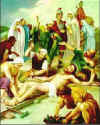
\includegraphics[width=2cm]{jalansalib_files/11_small.jpg}
\end{wrapfigure}
\subsection*{Perhentian XI\\
YESUS DIPAKU DI KAYU SALIB}

\BP{   Kami menyembah Dikau ya Tuhan dan bersyukur\\kepadaMu.}
\BU{   Sebab dengan salib suci, Engkau telah menembus dunia. } 

\BP{Mereka  mendorong   Puteraku,    dengan   kasar   higga    jatuh   ke tanah,   ke dua tanganNya ditarik di atas kayu salib. Dia membiarkan diri-Nya dipaku. Ketika mereka menembusi tangan dan kakiNya dengan paku besar, jeritan jiwaku tak dapat kutahan lagi menyaksikan kekejaman seperti itu lebih baik aku mati saja dari pada melihat perlakuan mereka terhadap Puteraku. Lalu mereka menegakkan salib, diatas salib itulah, Puteraku tergantung. Ia dihina. Ketika Puteraku bergulat dengan maut pada saat-saat terakhir hidupNya didunia ini melawan kuasa kegelapan, dosa dan ejekan caci maki yang pedas dari mereka. Tapi aku menyadari itulah bukti cinta Tuhan pada manusia, maka aku berdiri tenang sambil berdoa diam-diam.}

\BU{ Tuhan Yesus, betapa pedih derita  yang  Engkau  tanggung  sendiri  bagiku,  dan betapa besar kesedihan ibu-Mu, menyaksikan dan memandang Engkau sebagai Puteranya yang tunggal mati, karena cinta kepadaku, aku sadar akan cinta-Mu dan Engkau bersama ibu Maria siap dan rela untuk mengampuni aku segera setelah aku menyesal, dan bertobat atas kesalahan dan dosa-dosaku. Ampunilah dan bantulah aku ya Tuhan Yesus untuk selalu berbalik dari jalan kegelapan dosa-dosaku.}

\large\begin{itemize}\item[~]\it{Bapa Kami - Salam Maria}\end{itemize}\normalsize
\BP{Kasihanilah Tuhan, kasihanilah aku}
   \BU{Allah ampunilah aku orang berdosa.}

\begin{itemize}
\item[11.] \it{Bunda perawan yang suci\\bimbinglah aku anakmu\\
      ingin menyertaimu.
}\end{itemize}

\begin{wrapfigure}[0]{r}{2cm}
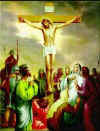
\includegraphics[width=2cm]{jalansalib_files/12_small.jpg}
\end{wrapfigure}
\subsection*{Perhentian XII\\
YESUS WAFAT DI SALIB}

\BP{   Kami menyembah Dikau ya Tuhan dan bersyukur\\kepadaMu.}
\BU{   Sebab dengan salib suci, Engkau telah menembus dunia.}

\BP{ Derita manakah yang lebih besar bagi seorang ibu,dari pada menyaksikan dengan mata sendiri kematian Anaknya. Aku yang telah melahirkan Putera ini ke dunia, dan menyaksikan Dia bertumbuh dewasa, sekarang berdiri tak berdaya dikayu salib. Ketika Dia menundukkan kepala-Nya, dan wafat.kesengsaraan-Nya sebagai manusia telah berakhir, namun penderitaanku bahkan meluap-luap. Namun aku sadar, semua ini harus terjadi dan aku harus menerimanya dalam iman Aku hanya dapat menangis dan berdoa;}

\BU{Yesus dan penyelamatku,kasihanilah aku atas segala akibat dosa-dosaku terhadap Mu selama ini, dan terhadap sesamaku. Terima kasih atas pengorbanan cintaMu dikayu salib yang begitu besar. Engkau sendiri mengatakan bahwa cinta yang benar   ialah menyerahkan nyawa bagi sahabat-sahabatMu. Ajarilah aku meneladani cintaMu dan cinta bunda-Mu Maria untuk hidup bagi sesamaku, dan tidak lagi menyia-nyiakan Engkau dalam diriku.}

\large\begin{itemize}\item[~]\it{Bapa Kami - Salam Maria}\end{itemize}\normalsize
\BP{Kasihanilah Tuhan, kasihanilah aku}
   \BU{Allah ampunilah aku orang berdosa.}

\begin{itemize}
\item[12.] \it{Betapa sedih hatimu\\melihat Putera meninggal\\
      tanpa hiburan Bapa.
}\end{itemize}

\begin{wrapfigure}[0]{r}{2cm}
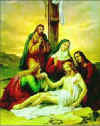
\includegraphics[width=2cm]{jalansalib_files/13_small.jpg}
\end{wrapfigure}
\subsection*{Perhentian XIII\\
JENASAH YESUS DITURUNKAN DARI SALIB}

\BP{   Kami menyembah Dikau ya Tuhan dan bersyukur\\kepadaMu.}
\BU{   Sebab dengan salib suci, Engkau telah menembus dunia.}

\BP{Para serdadu telah bubar semuanya, pekik sorak telah reda. Aku berdiri di bawah salib bersama salah seorang sahabat Puteraku, dan memandang tubuh yang tak bernyawa lagi, tubuh penyelamat kita. Lalu dua orang lelaki menurunkan jenasah Puteraku dari salib, dan menaruhnya di atas pangkuanku. Aku tenggelam dalam lautan duka yang hebat. Disinilah aku menunjukan cinta keibuanku dengan merangkul Puteraku penuh cinta dan cucuran air mata.Hidup Puteraku telah berakhir secara sadis dan tragis, yang juga membawa hidup baru bagi umat manusia. Ini semua harus terjadi, dan aku berdoa dalam cucuran air mata.}

\BU{Penyelamatku, sengsara-Mu telah berakhir  namun  hal itu masih saja terjadi, bila setiap kali aku memihak dan berbuat dosa dari pada kembali dan memilih Engkau. Akulah yang menyalibkan Engkau, sekarang ya Tuhan, aku sadar, aku mau setia dan mencintai-Mu dalam kehidupanku. Aku mohon juga pengampunan-Mu.     dan bantulah aku mencintai salib-Mu sehari-hari seturut teladan-Mu dan ibu-Mu.}

\large\begin{itemize}\item[~]\it{Bapa Kami - Salam Maria}\end{itemize}\normalsize
\BP{Kasihanilah Tuhan, kasihanilah aku}
   \BU{Allah ampunilah aku orang berdosa.}

\begin{itemize}
\item[13.] \it{Semoga darah penebus\\jadi pedoman hidupku\\
      di dalam dunia ini.
}\end{itemize}

\begin{wrapfigure}[0]{r}{2cm}
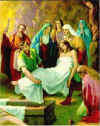
\includegraphics[width=2cm]{jalansalib_files/14_small.jpg}
\end{wrapfigure}
\subsection*{Perhentian XIV\\
YESUS DIMAKAMKAN}

\BP{   Kami menyembah Dikau ya Tuhan dan bersyukur\\kepadaMu.}
\BU{   Sebab dengan salib suci, Engkau telah menembus dunia.}

\BP{Kami mengantar jenasah  Yesus  Puteraku  di sebuah  taman, d imana di sana ada makam baru yang belum pernah ditempati oleh seorangpun. Aku sendiri yang mengatur semuanya disana, dengan cucuran air mata karena sedih dan bersukacita      atas kehendak Allah yang sudah terjadi. Sekali lagi aku memandang Yesus Puteraku yang sangat kucintai. Lalu aku keluar dari kubur. Mereka menutupnya dengan batu besar. Dan sebelum aku meninggalkan makam, aku sempat berpikir, aku sadar bahwa semua ini harus terjadi, untuk keselamatan dunia. Aku hanya berharap dalam iman akan janji-Nya sambil berdoa;}

\BU{Ya Tuhan Yesus, cinta-Mu telah terbukti atas dunia ini, Engkau sungguh-sungguh mencintai aku, orang yang berdosa ini. Dan tidak ada alasan lain, Engkau hanya berharap agar aku hidup baik dan hidup seturut rencana-Mu. Engkau tak pernah mengatakan bahwa hidup baik itu mudah. Tuhan, aku hendak meninggalkan dosa-     dosaku saat ini, dan hidup hanya untuk-Mu, dalam saudara-saudaraku.}

\large\begin{itemize}\item[~]\it{Bapa Kami - Salam Maria}\end{itemize}\normalsize
\BP{Kasihanilah Tuhan, kasihanilah aku}
   \BU{Allah ampunilah aku orang berdosa.}

\begin{itemize}
\item[14.] \it{Tolonglah aku bertekun\\agar kelak berbahagia\\
      bersama dengan Yesus.
}\end{itemize}

\end{document} 
